% 2008 年重庆卷理科第 16 题：三棱柱 ABC-A1B1C1 的 6 个顶点各装一个灯泡。
% 来源 PDF：gaokaomath-src/普通高考/2008/2008重庆理.pdf
% SHA-256：d3ca36cef73a00068b9c1a97ddb2f90bbc4f16b38459e380579090a02706d937
% 原页：2008重庆理.pdf 第 1 页（A3 三栏）第 2 栏，书页码 429。
% 绘制依据：按原页画出三棱柱的 9 条棱与 6 个顶点，A1B1C1 在下、ABC 在上。
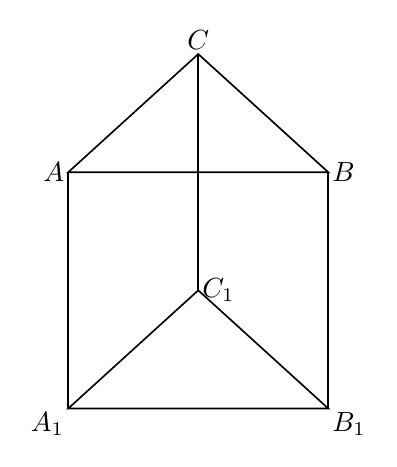
\begin{tikzpicture}[scale=1.5, semithick, every node/.style={inner sep=1.2pt}]
  \coordinate (A) at (0,2.0);
  \coordinate (B) at (2.2,2.0);
  \coordinate (C) at (1.1,3.0);
  \coordinate (A1) at (0,0);
  \coordinate (B1) at (2.2,0);
  \coordinate (C1) at (1.1,1.0);
  \draw (A) -- (B) -- (C) -- cycle;
  \draw (A1) -- (B1) -- (C1) -- cycle;
  \draw (A) -- (A1);
  \draw (B) -- (B1);
  \draw (C) -- (C1);
  \node[left] at (A) {$A$};
  \node[right] at (B) {$B$};
  \node[above] at (C) {$C$};
  \node[below left] at (A1) {$A_1$};
  \node[below right] at (B1) {$B_1$};
  \node[right] at (C1) {$C_1$};
\end{tikzpicture}
